\section{Theoretische Grundlagen}
\subsection{Allgemeines zu Interferenz und Kohärenz}
Überlagern sich zwei Lichtwellen kann es zur \texttt{Interferenz} kommen.
Diese äußert sich in destruktiver Interferenz (Auslöschung der Welle, keine Intensität) und konstruktiver Interferenz (Addition der Wellenextrema, verstärkte Intensität).
Eine wichtige Bedingung hierfür ist, dass die Wellen die gleiche Wellenlänge haben.
Genauer gesagt, für eine länger andauernde, stabile Interferenz, müssen beide Wellen kohärent sein.
\texttt{Kohärenz} beschreibt den Aspekt, dass die Wellenlänge zweier überlagernder Wellen über die Dauer der Kohärenzzeit gleich ist.
Die Kohärenzzeit wiederum ist die Zeit, über die sich die Welle nicht ändert.
Die Kohärenzzeit endet, sobald die Lichtquelle einen Phasensprung aussendet oder, seltener, wenn sich die Eigenschaften der Lichtwelle (Wellenlänge, Phase, etc.) der Lichtquelle ändert.
Andersherum bedeutet \texttt{zeitliche Kohärenz}, dass bei eine ausgekoppelte Teilwelle nach einiger Zeit kohärent zur Ursprungswelle zurückgeführt werden kann.
\texttt{Räumliche Kohärenz} liegt vor, wenn zwei ausgekoppelte Teilwellen trotz räumlicher Verschiebung miteinander interferieren können.
Der \texttt{Kohärenzgrad} stellt die Interferenzfähigkeit zweier Wellen dar.

\FloatBarrier
\subsection{Polarisation}
Die Polarisation einer Welle beschreibt der Auslenkungsrichtung der Wellen.
Bei zirkular polarisierten (Abb. \ref{fig:polarisation}, c) oder elliptisch polarisierten (Abb. \ref{fig:polarisation}, b) Lichtwellen dreht sich die Auslenkungsrichtung um die Bewegungsrichtung.
Die lineare Polarisation (Abb. \ref{fig:polarisation}, a) zeichnet sich durch eine gleichbleibende Auslenkungsrichtung senkrecht zu Ausbreitungsrichtung aus.
Wird linear polarisiertes Licht auf eine Grenzfläche gestrahlt, wechelwirkt es dort in zwei Ausprägungen (Abb. \ref{fig:linpol}).
Durch eine Grenzfläche wird ausschließlich der Anteil des linear polarisierten Lichts transmittiert, der eine zur Spiegelebene \textbf{p}arallele Auslenkungsrichtung hat und heißt entsprechend \texttt{p-polarisiert}.
Der reflektierte Anteil des Lichts hat eine ausschließlich zur Spiegelebene \textbf{s}enkrechte Auslenkungsrichtung und wird \texttt{s-polarisiert} genannt.
\begin{figure}[!ht]
	\centering
	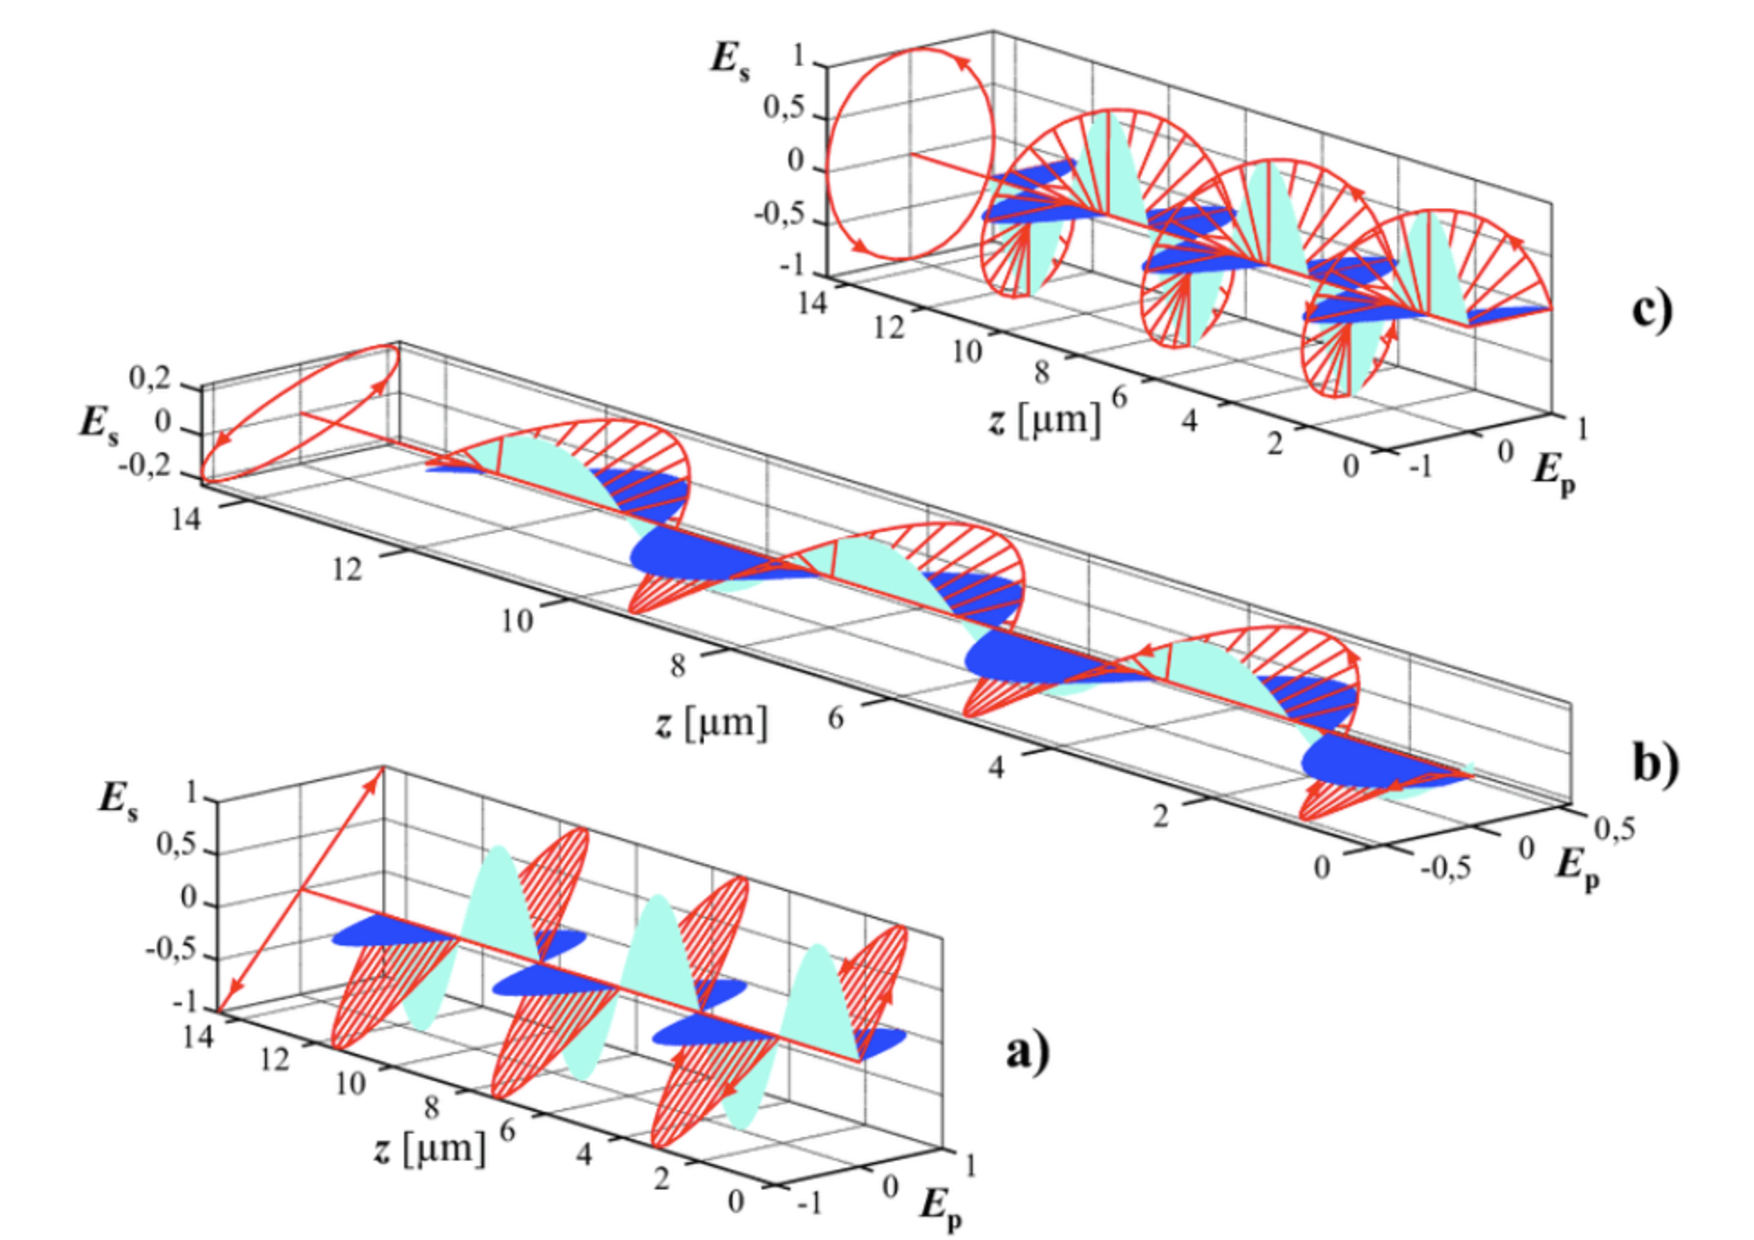
\includegraphics[width=\textwidth]{content/images/polarisation.pdf}
    \caption{Darstellungen der Polarisationsarten: Linear, zirkular und elliptisch \cite{diss-busk}.}
    \label{fig:polarisation}
\end{figure}

\begin{figure}[!ht]
	\centering
	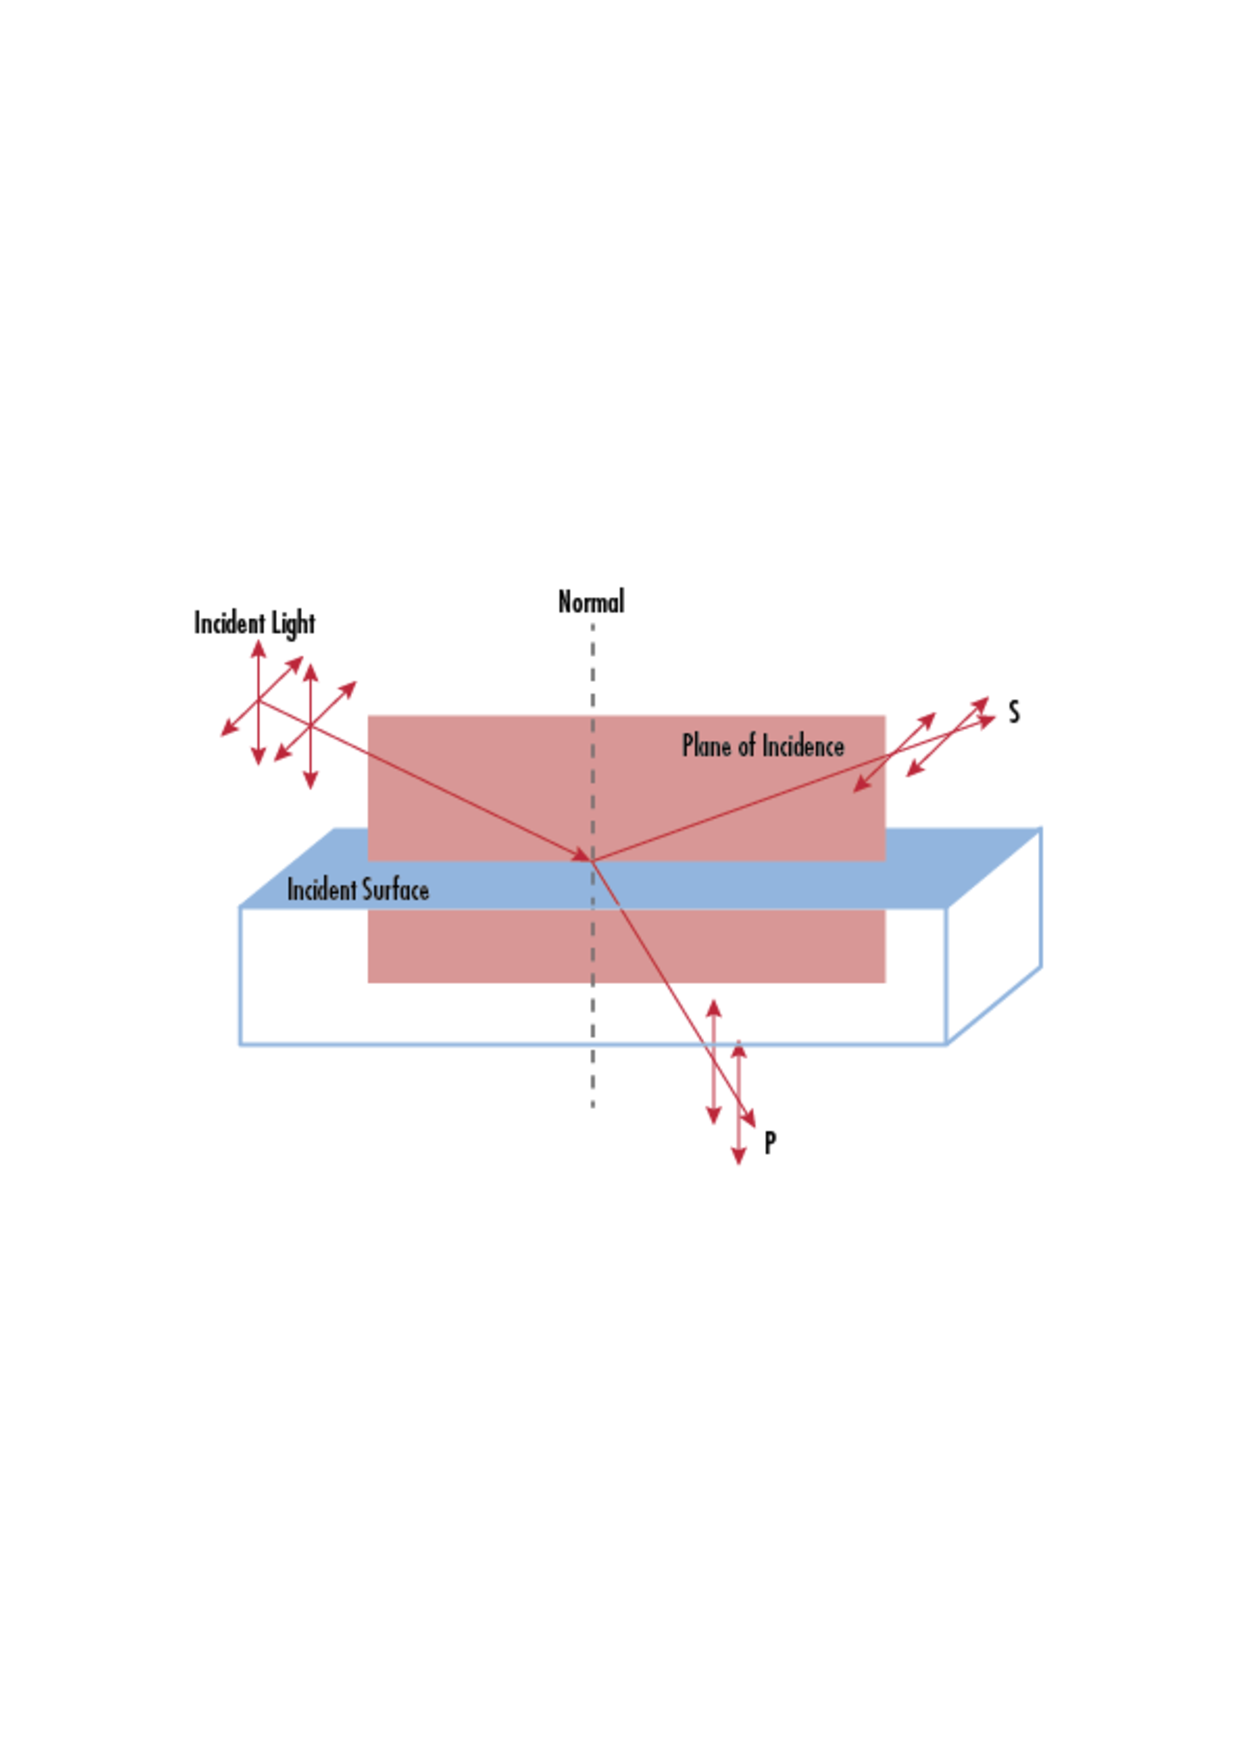
\includegraphics[width=0.6\textwidth]{content/images/sundppol.pdf}
    \caption{Polarisation von transmittierten und reflektierten Wellen \cite{edmund}.}
    \label{fig:linpol}
\end{figure}

%\begin{figure}[!ht]
%\begin{subfigure}[c]{0.50\textwidth}
%	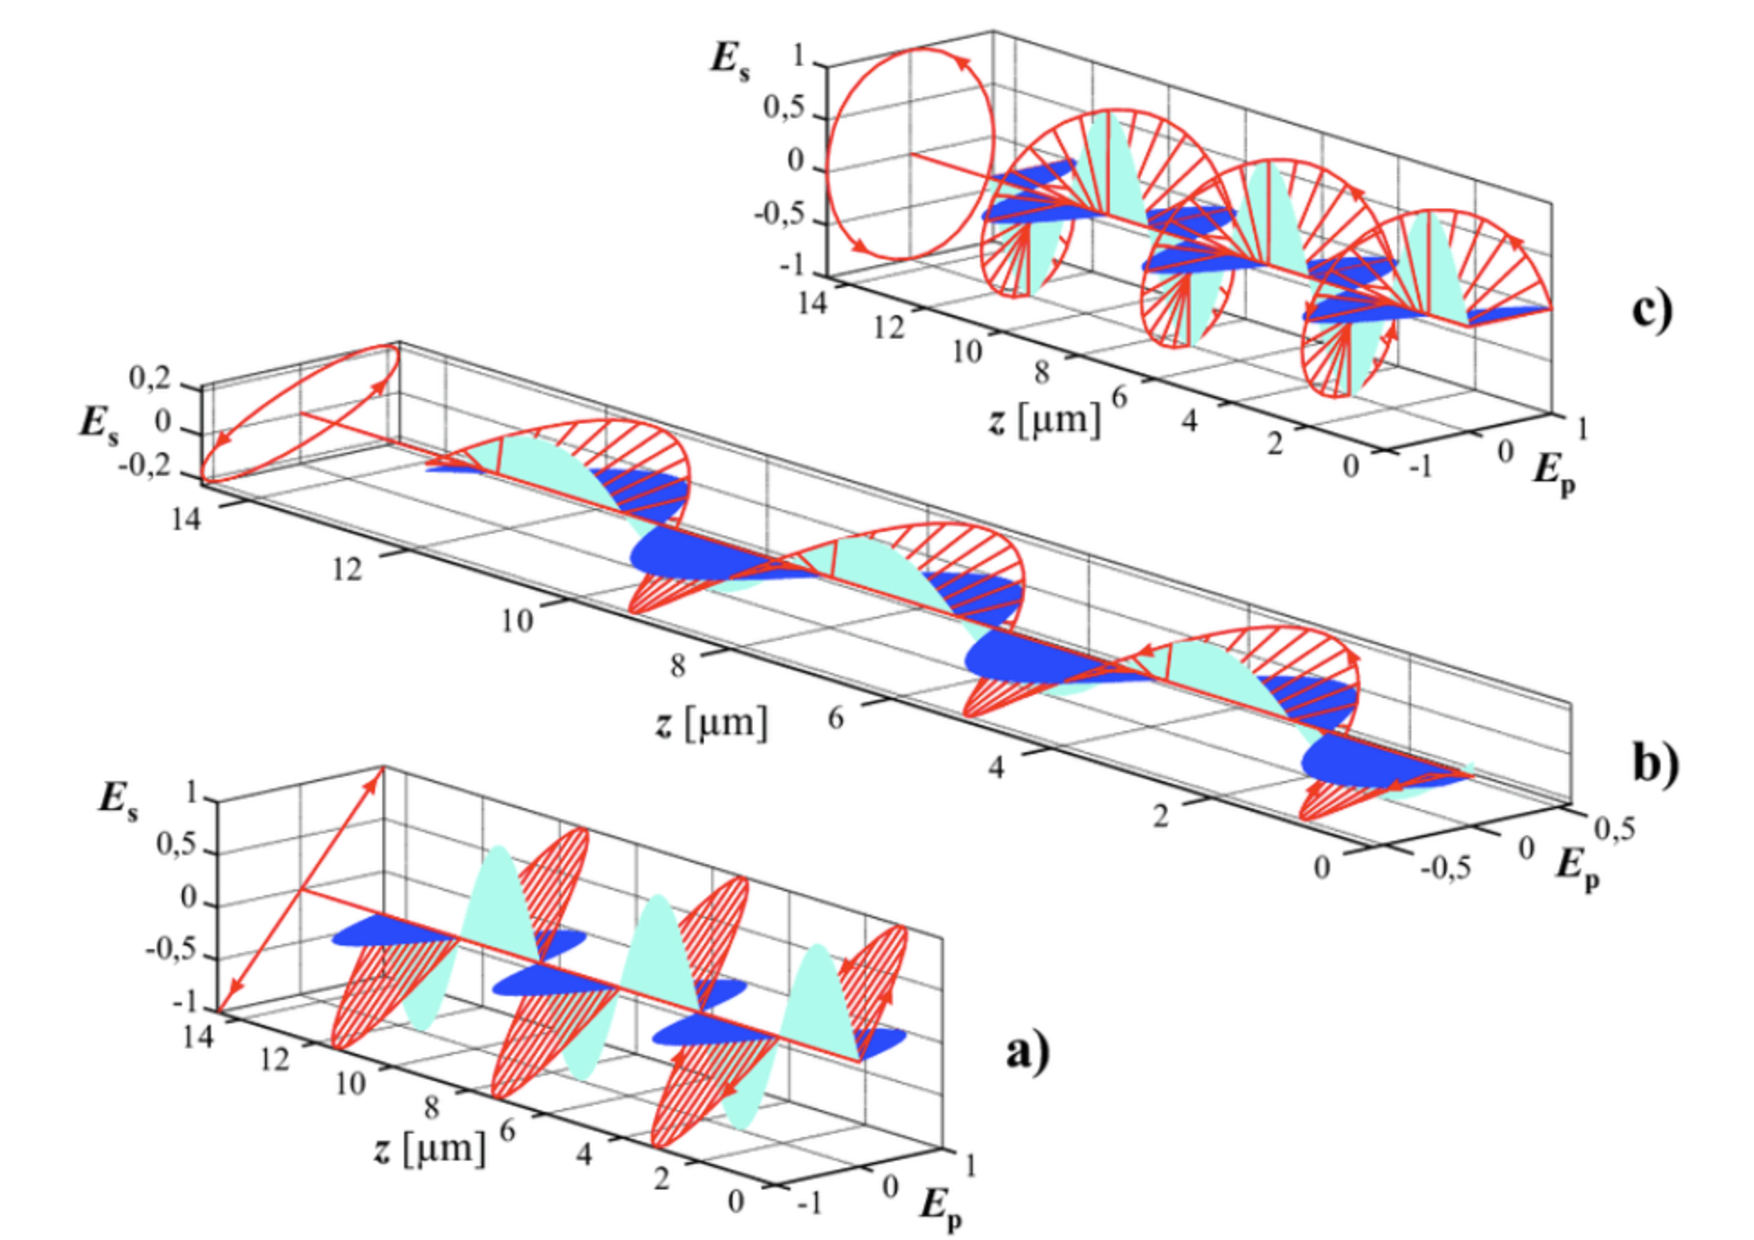
\includegraphics[width=\textwidth]{content/images/polarisation.pdf}
%    \caption{Darstellungen der Polarisationsarten: Linear, zirkular und elliptisch \cite{diss-busk}.}
%    \label{fig:polarisation}
%\end{subfigure}
%\hspace*{\fill}
%\begin{subfigure}[c]{0.50\textwidth}
%	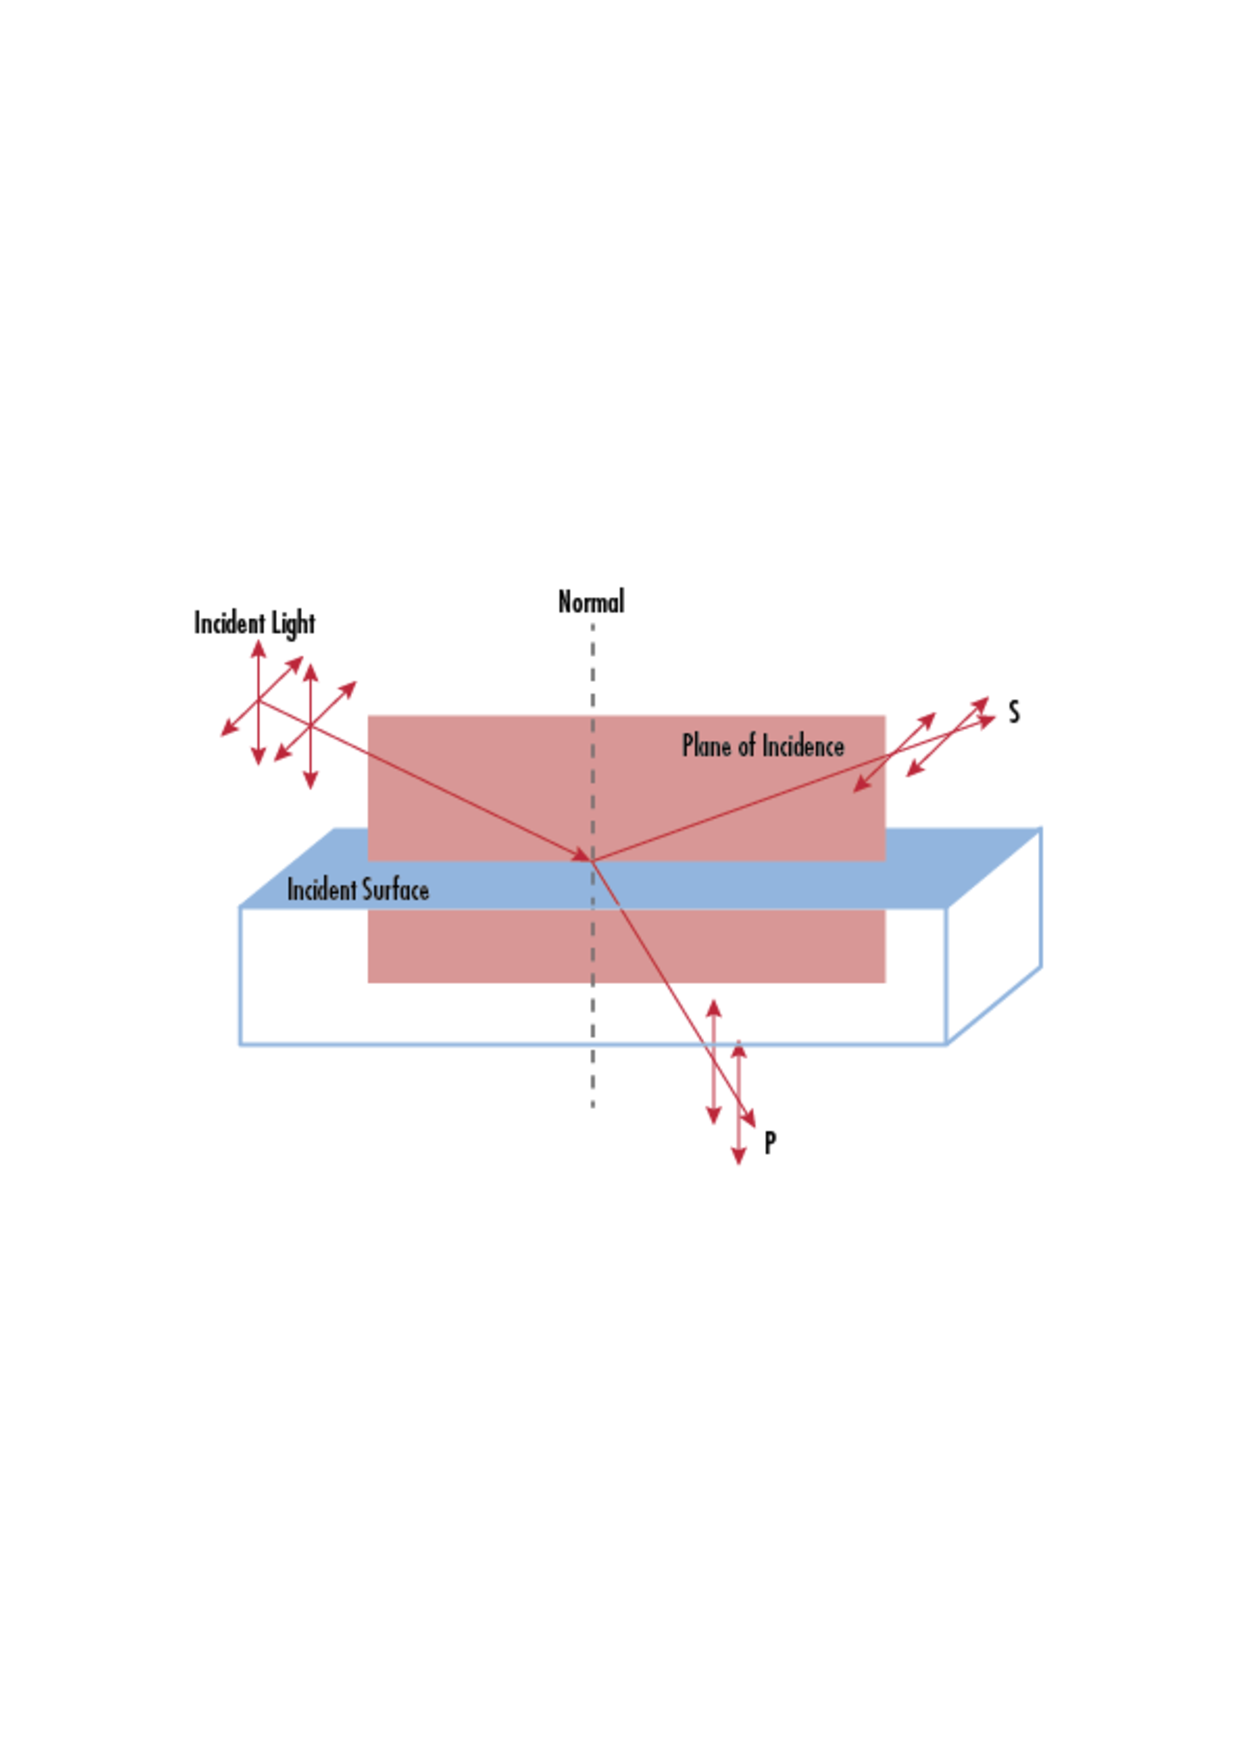
\includegraphics[width=\textwidth]{content/images/sundppol.pdf}
%    \caption{Polarisation von transmittierten und reflektierten Wellen \cite{edmund}.}
%    \label{fig:linpol}
%\end{subfigure}
%\end{figure}

Interferenzen können nur bei gleich polarisierten Wellen oder gleich polarisierten Wellenanteilen entstehen, da sich die elektrischen Felder sonst nicht aufheben können.
Entsprechen interferieren s-polarisiertes und p-polarisiertes Licht nicht miteinander, auch wenn beide Strahlen in der gleichen Ebene verlaufen.

\FloatBarrier
\subsection{Kontrast und Intensität}
Um die Qualität eines Interferenzbildes eines Interferometers anzugeben, wird der Kontrast $V$ (auch Sichtbarkeit, eng. \textit{visibility}) eingeführt:
\begin{equation}
	V = \frac{I_{\text{max}} - I_{\text{min}}} {I_{\text{max}} + I_{\text{min}}}.
	\label{eqn:kontrastohnewinkel}
\end{equation}
Hierbei ist $I_{\text{max}}$ die Intensiät eines Intensitätsmaximums des Interferenzbildes, $I_{\text{min}}$ entsprechend die Intensität der Interferenz am Minimum.
Die Intensität des Interferenzbildes ist über das zeitlichen Mittel der elektrischen Feldstärke $E$ vom Polarisationswinkel $\phi$ zwischen den Wellen abhängig.
Dabei sind die interferierenden Wellen allgemein wie folgt definiert:
\begin{equation*}
	E_{1} =  E_{0} \cos{\left( \phi \right)} \cos{ \left( \omega t \right) } 			\quad \quad \quad
	E_{2} =  E_{0} \sin{\left( \phi \right)} \cos{ \left( \omega t + \delta \right) }. 	\\
\end{equation*}
\begin{center}
	\tiny{$\omega \widehat{=} \text{Kreisfrequenz}, \delta \widehat{=} \text{Phasenverschiebung} $}
\end{center}
Über folgende Zwischenergebnisse der zeitlichen Mittelung über eine ganze Periode
\begin{align*}
	&	I 					 	\propto	 \langle |E_{1} + E_{2}|^2 \rangle = \langle |\underbrace{ \, E_{1}^2 \, }_{\substack{I_1}} + \underbrace{ \, E_{2}^2 \, }_{\substack{I_2}} + \underbrace{ \, 2 \, E_{1} \! \cdot \! E_{2} \, }_{\substack{\text{\tiny{Interferenzterm}}}} |\rangle \\
  	&	I_{1} 	\propto	 \langle E_1^2 \rangle = E_0^2  \cos^2{(\phi)}\\ % =\int^{\frac{2 \pi}{\omega}}_{0} \! E_0^2 \cos^2{(\phi)} \cos^2{(\omega t)} dt
	&	I_2 	\propto	 \langle E_2^2 \rangle = E_0^2  \sin^2{(\phi)} \\
	&	I_{\text{Int.}}	\propto	 \pm 2 E_0^2  \sin{(\phi)} \cos{(\phi)}\\
%  		I_{1}				&& 	\propto	 \langle E_1^2 \rangle = E_0^2 \pi \cos^2{(\phi)} 											&& \\ % =\int^{\frac{2 \pi}{\omega}}_{0} \! E_0^2 \cos^2{(\phi)} \cos^2{(\omega t)} dt
%		I_{2}				&& 	\propto	 \langle E_2^2 \rangle = E_0^2 \pi \sin^2{(\phi)} 											&& | \delta = n \pi, n \in \mathbb{Z} \\ %\int^{\frac{2 \pi}{\omega}}_{0} \! E_0^2 \sin^2{(\phi)} \cos^2{(\omega t + \delta)} dt
%  		I_{\text{Int.}} 	&& 	\propto	 \langle 2 E_1 E_2 \rangle &&\\ %= \langle 2 E_0^2 \sin{(\phi)} \cos{(\phi)} \cos{(\omega t )} \cos{(\omega t + \delta)}\rangle 															&& \\
%		I_{\text{Int.}}		 	\propto	 \langle 2 E_0^2 \sin{(\phi)} \cos{(\phi)} \cos{(\omega t )} \bigl[ \cos{(\omega t)} \cos{(\delta )} - \sin{(\omega t)} \sin{(\delta)} \bigr]\rangle 								&& | \cos{(\delta)}= \pm 1, \sin{(\delta)}=0 \\
%		 										&& \\ %\pm \int^{\frac{2 \pi}{\omega}}_{0} \! 2 E_0^2 \sin{(\phi)} \cos{(\phi)} \cos^2{(\omega t )} dt =
\end{align*}
ergibt sich die Intensität eines Minimums ($\delta = n \pi$, $n \in \mathbb{Z}$) bzw. Maximums ($\delta=2n\pi$, $n \in \mathbb{Z}$) zu:
\begin{equation*}
	I_{\text{max/min}} 	= I_1+I_2+I_{\text{Int.}} \quad \propto I_{\text{ges}} \left(1 \pm 2 \cos{(\phi)} \sin{(\phi)}\right).
	\label{eqn:intensity}
\end{equation*}
Damit liegt dem Kontrast auch eine $\phi$-Abhängigkeit zugrunde:
\begin{equation}
	V(\phi) \propto = 2 \cos{(\phi)} \sin{(\phi)} = \sin{(2\phi)}. % \frac{(1+2\cos{(\phi)} \sin{(\phi)}) - (1-2\cos{(\phi)} \sin{(\phi)})} {(1+\cos{(\phi)} \sin{(\phi)}) + (1-2\cos{(\phi)} \sin{(\phi)})} \quad
	\label{eqn:kontrastmitwinkel}
\end{equation}

\FloatBarrier
\subsection{Brechungsindices von Gasen und Festkörpern}
\paragraph{Brechungsindex von Gas}
Ähnlich wie Gläser können auch Gase Lichtwellen brechen und reflektieren (z.B. Fata Morgana).
So haben sie einen Brechungsindex, der mit dem Gasdruck und der Temperatur skaliert.
Im Vergleich zu einer Lichtwelle, die durch das Vakuum läuft, ergibt sich für die Lichtwelle in Gas eine Phasenverschiebung $\Delta \delta$.
Somit lässt sich bei zwei Lichtwellen, von denen eine über die Länge $L$ durch eine evakuierte Kammer läuft und die andere über die Länge $L$ weiter durch das Gas verläuft, die Phasenverschiebung in Abhängigkeit des Brechungsindex $n$ des Gases ausdrücken:
\begin{equation}
	\Delta \delta = \frac{2 \pi L}{\lambda_{0}} (n-1) .
\end{equation}
\begin{center}
	\tiny{$\L \widehat{=} \text{Länge der Kammer}, \lambda_{0}{=} \text{Vakuum-Wellenlänge}, n \widehat{=} Brechungsindex des Gases$}
\end{center}
Die Anzahl der Interferenzmaxima in einem Intervall verschiedener Phasenverschiebungen $\Delta \delta$ berechnet sich wie folgt:
\begin{equation*}
	M = \frac{\Delta \delta}{2 \pi} \Rightarrow M = \frac{L (n-1)}{\lambda_{0}} \Leftrightarrow n = \frac{M \lambda_{0}}{L} +1.
%	\label{eqn:brechungsindex_gas}
\end{equation*}
Der Brechungsindex ist über das Lorentz-Lorenz-Gesetz mit dem Druck und der Temperatur des Gases verbunden und kann über eine Taylorentwicklung um $n\approx 1$ wie folg genähert werden:
\begin{equation}
	\frac{n^2-1}{n^2+2} = \frac{A p }{R T} \approx  \frac{2}{3} (n-1) + \mathcal{O}(n^2) \quad \Leftrightarrow n(p) \approx \frac{3A p}{2R T} +1.
	\label{eqn:gas}
\end{equation}

\paragraph{Brechungsindex von Glas}
Wird ein Lichtstrahl durch eine planparallele Platte geschickt, wird er zweimal um den gleichen Winkel in gegensätzliche Richungen gebrochen und behält so global seine Ausbreitungsrichtung bei, wird jedoch seitlich verschoben.
Die Brechung ist abhängig vom Drehwinkel $\theta$.
Läuft ein Teilstahl durch eine planparallele Platte, und ein zweiter Teilstrahl nicht, ergibt sich eine Phasenverschiebung zwischen den beiden Strahlen:
\begin{equation*}
	\Delta \delta = \frac{2 \pi T}{\lambda_0} \left[ \frac{n-1}{2n} \, \theta^2 + \mathcal{O}(\theta^4) \right].
\end{equation*}
Im Falle dieses Versuchs sind es zwei um konstant $\SI{20}{°}$ gegeneinander gekippte Glasplatten, die um den Drehwinkel $\theta$ gedreht werden:
\begin{equation*}
	\Delta M = \Delta 2 \, \cdot \frac{\Delta \delta}{2 \pi} = 2 \cdot \frac{T}{\lambda_{0}} \frac{n-1}{2n} \, (\theta_1^2 - \theta_2^2)
\end{equation*}
\FloatBarrier
